\documentclass[a4paper]{article}

%% Language and font encodings
\usepackage[english]{babel}
\usepackage[utf8x]{inputenc}
\usepackage[T1]{fontenc}

%% Sets page size and margins
\usepackage[a4paper,top=3cm,bottom=2cm,left=3cm,right=3cm,marginparwidth=1.75cm]{geometry}

%% Useful packages
\usepackage{amssymb, graphicx, amsmath, amsthm,mathabx}
\usepackage[colorinlistoftodos]{todonotes}
\usepackage[colorlinks=true, allcolors=blue]{hyperref}

\newtheorem{theorem}{Theorem}
\newtheorem{definition}{Definition}
\newtheorem{proposition}{Proposition}
\newtheorem{lemma}{Lemma}

\title{Notes: Canonical Transform}
\author{Héctor Andrade Loarca, Philipp Petersen}

\begin{document}
\maketitle

\begin{abstract}
In this notes we present the canonical shearlet transform associated to the space of the two dimensional tomography. The main reason of this construction is the characterization of the Wavefront set of the sinogram of a tomographic image by studying the decay rate of its shearlet coefficients, which at the same time characterizes the Wavefront set of the original image. 
\end{abstract}

\section{Two dimensional electron tomography}

Tomography is a process of imaging by sections or sectioning of a speciment of interest, through the use of any kind of penetrating wave. This method is used in radiology, archaeology, biology, geophysics, materials science, and other areas of science. In many cases the production of the images based on tomography arise after solving an inverse problem, known as tomographic reconstruction, generally ill-posed. 

\bigskip

There exist different methods of tomography acquisition, in this work we will study the measurment setting associated with the so called X-ray transform (or parallel beam transform), that measures the attenuation coefficient of an specimen $f\in L^2(\mathbb{R}^n)$ by the values of its integral along different straight lines. In two dimensions the X-ray transform coincides with the Radon transform.

\begin{definition}[Radon Transform]
\label{Radondef}
Let $f\in L^2(\mathbb{R}^2)$, $\theta\in [0,2\pi)$ and $s\in\mathbb{R}$ then the Radon transform of $f$ along the line $L(\theta,s) = \{ (x,y)\in\mathbb{R}^2 : x cos\theta + y \sin\theta = s\}$ is given by the integral
\begin{equation}
\label{eq:Radoneq1}
\mathcal{R}f (L)=\mathcal{R}f(\theta,s)=\iint_{(x,y)\in L} f(x,y)dS = \int_{-\infty}^{\infty}\int_{-\infty}^{\infty} f(x,y) \delta (x\cos\theta+y\sin\theta-s)dxdy
\end{equation}
to this definition of Radon transform we refer as the sinogram and is the one we are gonna focus on. Although one could also use the next definition
\begin{equation}
\label{eq:Radoneq2}
\mathcal{R}  f(u,s) := \int_{x_2\in\mathbb{R}} f(u-sx_2,x_2)dx_2
\end{equation}
\end{definition}

In Figure~\ref{fig:Sheep-Logan-Phantom} one can see the Sheep-Logan phantom, which is a standard test image, that serves as the model of a human head in the developing and testing of image reconstruction algorithms. Figure~\ref{fig:Sheep-Logan-Phantom-Measured} show the measured lines of the phantom used for the Radon transform, and finally in Figure~\ref{fig:Sinogram} one can finally see the sinogram o Radon transform of the phatom.

\begin{figure}[h!]
\centering
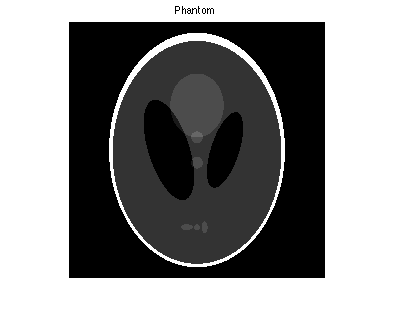
\includegraphics[width = 0.55\textwidth]{./phantom.png}
\caption{Shepp-Logan phantom}
\label{fig:Sheep-Logan-Phantom}
\end{figure}

\begin{figure}[h!]
\centering
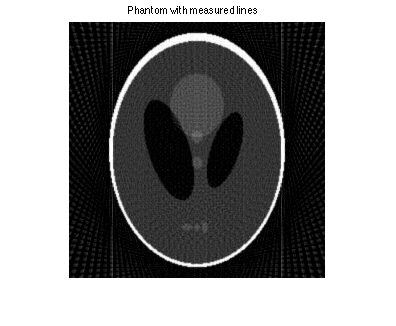
\includegraphics[width = 0.55\textwidth]{./phantom_measured.png}
\caption{Shepp-Logan phantom with measured lines}
\label{fig:Sheep-Logan-Phantom-Measured}
\end{figure}

\begin{figure}[h!]
\centering
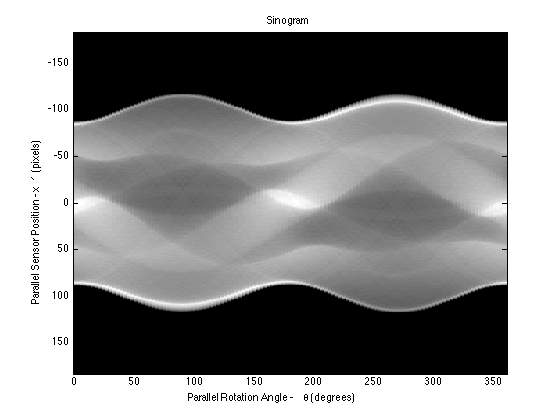
\includegraphics[width = 0.55\textwidth]{./sinogram.png}
\caption{Sinogram}
\label{fig:Sinogram}
\end{figure}

\bigskip

As one can see the sinogram and the original picture are form of singularities of different types. This problem is ill-posed since its associated inverse (Filtered Back Projection) is unbounded, so one would need to perform a regularization method and extra information of $f$ can play and important role when trying to regularize \cite{IllPosedDLOektem}. We would like to use information about the regularity of $f$ as extra information in the regularization of the problem. The concepts of singularity and regularity can be generalized to all distributions, the theory behind this is known as microlocal regularity theory. In this work we will explain a method to extract regularity information of a function using shearlet frames, when one knows just its Radon transform. 

\section{Microlocal regularity}

\begin{definition}[$N$-regular point and $N$-regular directed point]
Let $N\in\mathbb{R}$ and $f$ a distribution on $\mathbb{R}^2$. We say that $x\in\mathbb{R}^2$ is a $N-$regular point if there exists a neighbourhood $U_x$ of $x$ such that $\Phi \psi\in C^N$, where $\Phi$ is a smooth cutoff function with $\Phi\equiv 1$ on $U_x$. 

Furthermore we call $(x,\lambda)$ and $N$-regular directed point if there exists a neighbourhood $U_x$ of $x$, a smooth cutoff function $\Phi$ with $\Phi\equiv 1$ on $U_x$ and a neighbourhood $V_{\lambda}$ of $\lambda$ such that

\begin{equation}
\label{eq:N-reg-direc}
(\Phi f)^{\wedge}(\eta)=O((1-|\eta|)^{-N}) \quad\text{for all}\quad \eta=(\eta_1,\eta_2)\quad \text{such that}\quad \frac{\eta_2}{\eta_1}\in V_{\lambda}
\end{equation}
\end{definition}

\bigskip

The $N-$Wavefront Set $WF^N(f)$ is defined as

\begin{equation}
\label{eq:N-wavefront-set}
WF^N(f):=\{(x,\lambda)\in \mathbb{R}^2\times(\mathbb{R}^2\setminus\{0\}): (x,\lambda)\quad \text{is not a $N-$regular directed point of f}\}
\end{equation}

\textbf{The Wavefront Set} $WF(f)$ is defined as 

\begin{equation}
\label{eq:Wavefront-set}
WF(f)=\bigcup_{N>0}WF^N(f)
\end{equation}

Notice that if $(x,\lambda)\in WF(f)$ then $x$ is a singular point of $f$, then the Wavefront Set ha the information of the singular domain of $f$ and the direction to where the singularities move. The directional information that one can extract using the Radon transform, can be used to characterize the Wavefront Set of a function, this using the definition at equation~\ref{eq:Radoneq2}.

\begin{theorem}[Projection Slice Theorem, \cite{WaveFrontSetGrohs}]
\label{thm:proj-slice}
Let $f$ be a tempered distribution, then
$$
(\mathcal{R}f(u,s))^{\wedge}(\omega)=\hat{f}(w(1,s))
$$
Therefore, $(x,\lambda)$ is an $N-$regular directed point is that
$$
(\mathcal{R}\Phi f(u,s))^{\wedge}(\omega)=O(|\omega|^{-N}) \quad \text{and}\quad s\in V_{\lambda}
$$
\end{theorem}

In \cite{Ozan-tomography} Ozan \"Otkem, et al.\ presented a relation between the $N-$Wavefront Set of a function and the $(N+1/2)-$Wavefront Set of its Radon transform. Also, in \cite{WaveFrontSetGrohs} Philipp Grohs presented a method of Wavefront Set Resolution using Continuous Shearlet Frames. The next is our goal:

\bigskip

\textbf{We want to transfer the information of the Wavefront set of a function using Shearlet Frames, when we just know its Radon transform.}


\section{Shearlets in Sinogram Space}

As one can refer to Equation~\ref{eq:Radoneq1}, the Radon transform of a function $\mathcal{R}f(x_1,x_2)$, where $(x_1,x_2)\in [0,2\pi)\times \mathbb{R}$ and it is $2\pi$-periodic in the $x_1$-direction, so in order to be able to use Shearlet Frames in the Radon Transform of a function, we would need first to construct a Shearlet Transform on $L^2_{2\pi-x_1}([0,2\pi)\times \mathbb{R})$ of square integrable functions on $[0,2\pi)\times \mathbb{R}$ that are also $2\pi$-periodic in $x_1$-direction. 
\bigskip 

We recall that given $(a,s,t)\in\mathbb{R}_{+}\times\mathbb{R}\times\mathbb{R}^2$, the classical shearlet transform of a function $f\in L^2(\mathbb{R}^2)$ associated to the generating function $\psi\in L^2(\mathbb{R}^2)$ is given by 

\begin{equation}
\label{eq:class_shear}
\langle f, \psi_{a,s,t}\rangle = \int_{\mathbb{R}^2} f(x)\overline{\psi_{a,s,t}(x)}dx
\end{equation}

where the shearlet system is given by

$$
\mathcal{SH}(\psi)=\{\psi_{a,s,t}(x):=a^{-3/4}\psi(S_sA_ax-t):(a,s,t)\in\mathbb{R}_+\times\mathbb{R}\times\mathbb{R}^2\}
$$

and the scaling matrix $A_a$ and shearing matrix $S_s$ are given by

$$
A_a := \left( \begin{matrix} a & 0 \\ 0 & a^{1/2}\end{matrix}\right), \quad S_s := \left(\begin{matrix} 1 & s \\ 0 & 1 \end{matrix}\right)
$$

Under some conditions on the generating function $\psi$, like the case of \textbf{\textit{classical shearlets}} \cite[p.~19]{ShearletsGitta}, the shearlet system will form a frame , in some cases (band-limited shearlets) one has even tight frames.

\bigskip

Our approach will be based on the so called \textbf{\textit{cone-adapted shearlet system}} generated by three functions $\phi,\psi,\tilde{\psi}\in L^ 2(\mathbb{R}^2)$, parameters $(a,s,t)\in\mathbb{R}_{+}\times\mathbb{R}\times\mathbb{R}^2$, the corresponding scaling and shearing matrices $A_a$ and $S_s$ and a sampling matrix $M_c=\text{diag}(c_1,c_2)$, where $c_1,c_2\in\mathbb{R}$.

\bigskip

In this setting the frequency domain is divided in specific areas distributed in two high-frequency cones and one low-frequency squared section; the horizontal cone is covered by elements $\psi_{a,s,t}(x)=a^{-3/4}\psi(S_sA_ax-M_ct)$, similarly the vertical cone is covered by elements of the form $\tilde{\psi}_{a,s,t}$, and finally the low-frequency section covered by a low pass filter elements of the form $\varphi_t = \varphi(x-c_1t)$. As well as the classical shearlets, the cone-adapted shearlets form a frame of $L^2(\mathbb{R}^2)$ under some conditions on the generating functions; the big difference between this two systems is that the later have a more optimal tiling of the frequency domain. The cone-adapted shearlet system generated by the functions $\varphi,\psi,\tilde{\psi}$ and sampling vector $c=(c_1,c_2)$ will be denote as $\mathcal{SH}(\varphi,\psi,\tilde{\psi};c)$, for a deeper analysis of this construction we refer to \cite{ConstructCompactShear}.

\bigskip

\begin{figure}[h!]
\centering
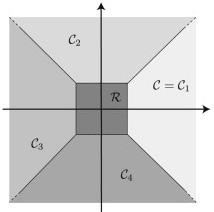
\includegraphics[width = 0.35\textwidth]{./cones.jpg}
\caption{Frequency domain cones}
\label{fig:Cones}
\end{figure}

As we already mentioned at the beginning of the section, the space associated to the sinogram of a function can be represented by the space 

$$
\begin{aligned}
L^2_{2\pi-x_1}([0,2\pi)\times\mathbb{R}):= \{ f:[0,2\pi)\times\mathbb{R}\longrightarrow \mathbb{R} &\bigg| \int_{[0,2\pi)\times\mathbb{R}}|f(x_1,x_2)|^2dx_1dx_2<\infty, \\
& f(x_1,x_2)=f(x_1+2\pi,x_2)\forall (x_1,x_2)\in [0,2\pi)\times\mathbb{R} \}
\end{aligned}
$$

We would like to construct a shearlet system that forms a frame for this space, the domain of the functions in this space is bounded (constraint in the infinte band $[0,2\pi]\times \mathbb{R}$), moreover one needs to have periodic conditions in the boundaries $x_1=0$ and $x_1=2\pi$. Our construction will be based mainly on three concepts: 
\begin{itemize}
\item Compactly supported shearlet frames.
\item Periodic summation.
\item Shearlets in bounded domains.
\end{itemize}

Broadly speaking we need to construct a shearlet system of periodic functions on a bounded domain, and for that one need first to construct compactly supported elements which form a frame. In the following subsections we are gonna explain this concepts to finally construct the desired system.

\subsection{Compactly supported shearlets}

We will to follow the construction of shearlet frames on bounded domains proposed by Kutyniok et al. \cite{ShearBounded} and for that we first need to construct a compactly supported shearlet frame. As we already mentioned before there are known cases of shearlet systems on $L^2(\mathbb{R}^2)$ that also form a frame for this space. For instance, the shearlet systems generated by classical shearlets and form a Parseval frame (therefore tight), but their elements are band-limited, therefore they cannot be compactly supported in the spatial domain. One would like then to have a general result of cone-adapted shearlet systems which are compactly supported and form a frame for $L^2(\mathbb{R}^2)$.

\bigskip

Following the construction proposed by Kutyniok et al. \cite{ConstructCompactShear} for $\varphi,\psi,\tilde{\psi}\in L^2(\mathbb{R})^2$, lets define $\Theta :\mathbb{R}^2\times\mathbb{R}^2\longrightarrow \mathbb{R}$ by

$$
\Theta(\xi,\omega):= |\hat{\varphi}(\xi)||\hat{\varphi}(\xi+\omega)|+\Omega_1(\xi,\omega)+\Theta_2(\xi,\omega)
$$

where

$$
\Theta_1(\xi,\omega)=\sum_{j\geq 0}\sum_{|k|\leq \lceil 2^{j/2}\rceil}|\hat{\psi}(S_k^{\intercal}A_{2^{-j}}\xi)||\hat{\psi}(S_k^{\intercal}A_2^{-j}\xi+\omega)|
$$

and

$$
\Theta_2(\xi,\omega)=\sum_{j\geq 0}\sum_{|k|\leq \lceil 2^{j/2}\rceil}|\hat{\tilde{\psi}}(S_k\tilde{A}_{2^{-j}}\xi)||\hat{\tilde{\psi}}(S_k\tilde{A}_{2^{-j}}\xi+\omega)|
$$

Also, for $c=(c_1,c_2)\in(\mathbb{R}_+)^2$, let
$$
\begin{aligned}
R(c)=\sum_{m\in\mathbb{Z}^2\setminus\{0\}}(&\Gamma_0(c_1^{-1}m)\Gamma_0(-c_1^{-1}m))^{1/2}+(\Gamma_1(M_c^{-1}m)\Gamma_1(-M_c^{-1}m))^{1/2}\\
&+(\Gamma_2(\tilde{M}_c^{-1}m)\Gamma_2(-\tilde{M}_c^{-1}m))^{1/2},
\end{aligned}
$$

where

$$
\Gamma_0(\omega)=\underset{\xi\in\mathbb{R}^2}{\text{ess}\text{sup}}|\hat{\varphi}(\xi)||\hat{\varphi}(\xi+\omega)| \quad \text{and} \quad \Gamma_i(\omega)=\underset{\xi\in\mathbb{R^2}}{\text{ess}\text{sup}}\Theta_i(\xi,\omega)\quad\text{for i=1,2}
$$

Where $\text{ess}\text{sup}$ is the essential supremum, which for a function $f\in L^2(\mathbb{R}^2)$ is defined as

$$
\underset{\xi\in\mathbb{R}^2}{\text{ess}\sup}f(x)=\inf\{a\in\mathbb{R}:\mu(\{\xi\in\mathbb{R}^2: f(\xi)>a\})=0\}
$$

where $\mu$ is the standard measure of $L^2(\mathbb{R}^2)$. Intuitively the essential supremum is the supremum of a function when we ignore sets of measure zero where the function might be unbounded. Similarly one can define the essential infimum as

$$
\underset{\xi\in\mathbb{R}^2}{\text{ess}\inf}f(x)=\sup\{b\in\mathbb{R}:\mu(\{\xi\in\mathbb{R}^2: f(\xi)<b\})=0\}
$$

\bigskip

With this concepts already defined we are ready to state general sufficient conditions for the construction of shearlet frames.

\bigskip

\begin{theorem}[\cite{ConstructCompactShear}]
\label{thm:suff_shear_frame}
Let $\varphi,\psi\in L^2(\mathbb{R}^2)$ be such that
$$
|\hat{\varphi}(\xi_1,\xi_2)|\leq C_1\cdot\min\{1,|\xi_1|^{-\gamma}\}\cdot\min\{1,|\xi_2|^{-\gamma}\}
$$

and

$$
|\hat{\psi}(\xi_1,\xi_2)|\leq C_2\cdot\min\{1,|\xi_1|^{\alpha}\}\cdot\min\{1,|\xi_2|^{-\gamma}\}\cdot \min\{1,|\xi_2|^{-\gamma}\}
$$
for some positive constants $C_1,C_2<\infty$ and $\alpha>\gamma>3$. Define $\tilde{\psi}(x_1,x_2)=\psi(x_2,x_1)$, and let $L_{\inf},L_{\sup}$ be defined by

$$
L_{\inf}(\omega)=\underset{\xi\in\mathbb{R}^2}{\text{ess}\inf}\Theta(\xi,0) \quad \text{and} \quad L_{\sup}=\underset{\xi\in\mathbb{R}^2}{\text{ess}\sup}\Theta(\xi,0)
$$

Then there exists a sampling parameter $c=(c_1,c_2)\in(\mathbb{R}^+)^2$ with $c_1=c_2$ such that $\mathcal{SH}(\varphi,\psi,\tilde{\psi};c)$ forms a frame for $L^2(\mathbb{R}^2)$ with frame bounds $A$ and $B$ satisfying

$$
0<\frac{1}{|\text{det}M_c|}[L_{\inf}-R(c)]\leq A\leq B \leq \frac{1}{|\text{det}M_c|}[L_{\sup}+R(c)]\leq \infty
$$
\end{theorem}

\bigskip

For the proof of this theorem we refer to \cite{ConstructCompactShear}. It is easy to show that band-limited shearlets obey this theorem, although it is harder in general to construct compactly supported shearlets that satisfy Theorem~\ref{thm:suff_shear_frame} and that form a frame for $L^2(\mathbb{R}^2)$. One can find various examples of compactly supported shearlets in \cite{ConstructCompactShear}, for its characteristics and simplicity we are gonna use the construction presented in the following theorem.

\begin{theorem}[\cite{ConstructCompactShear}]
\label{thm:compact_shear_construct}
Let $K,L>0$ be such that $L\geq 10$ and $\frac{3L}{2}\leq K\leq 3L-2$, and define a shearlet $\psi\in L^2(\mathbb{R}^2)$ by

$$
\hat{\psi}(\xi)=m_1(4\xi_1)\hat{\varphi}(\xi_1)\hat{\varphi}(2\xi_2), \quad \xi=(\xi_1,\xi_2)\in\mathbb{R}^2,
$$

where $m_0$ is the low-pass filter satisfying

$$
|m_0(\xi_1)|^2=(cos(\pi\xi_1))^{2K}\sum_{n=0}^{L_1}\left( \begin{matrix} K-1+n \\ n \end{matrix}\right)(sin(\pi\xi))^{2n}, \quad \xi_1\in\mathbb{R}
$$

$m_1$ is the associated bandpass filter defined by

$$
|m_1(\xi_1)|^2=|m_0(\xi_1+1/2)|^2, \quad \xi_1\in\mathbb{R}
$$

and $\varphi$ is the scaling function given by

$$
\hat{\varphi}(\xi_1)=\prod_{j=0}^{\infty}m_0(2^{-j}\xi_1), \quad \xi\in\mathbb{R}
$$

Then there exists a sampling constant $\hat{c}_1>0$ such that the shearlet system $\Psi(\psi;c)$ forms a frame for $\check{L}^2(\mathcal{C}_1\cup\mathcal{C}_3):=\{f\in L^2(\mathbb{R}^2): \text{supp} \hat{f}\subset \mathcal{C}_1\cup\mathcal{C}_3\}$ (where $\mathcal{C}_1$ and $\mathcal{C}_3$ are the horizontal cones in Figure~\ref{fig:Cones}) for any sampling matrix $M_c$ with $c=(c_1,c_2)\in (\mathbb{R}_+)^2$ and $c_2\leq c_1\leq \hat{c}_1$.
\end{theorem}

\bigskip

Since the proof of this theorem is not the main interest of this work we refer to \cite{ConstructCompactShear} for the proof. It is worth to notice that Theorem~\ref{thm:compact_shear_construct} but Theorem~\ref{thm:suff_shear_frame} assumes that one has uniform sampling, i.e. the sampling constants $c_1$ and $c_2$ coincides, but this results is easy to generalize to non-uniform sampling ($c_1\neq c_2$), we refer again to \cite{ConstructCompactShear} for the specific bounds estimates.

\bigskip

By construction the shearlet generators proposed in Theorem~\ref{thm:compact_shear_construct} are compactly supported (and therefore all the elements of the generated system), but they are frame just for $\check{L}^2(\mathcal{C}_1\cup\mathcal{C}_3)$; even though one can easily construct shearlet frames for the whole space $L^2(\mathbb{R}^2)$ as follows.

\bigskip

\begin{theorem}[\cite{ConstructCompactShear}]
\label{thm:whole_frame}
Let $\psi\in L^2(\mathbb{R}^2)$ be the shearlet with associated scaling function $\varphi_1\in L^2(\mathbb{R})$ both introduced in Theorem 2, and set $\varphi(x_1,x_2)=\varphi(x_1)\varphi(x_2)$ and $\tilde{\psi}(x_1,x_2)=\psi(x_2,x_1)$. Then the corresponding shearlet system $\mathcal{SH}(\varphi,\psi,\tilde{\psi};c)$ forms a frame for $L^2(\mathbb{R}^2)$ for any sampling matrices $M_c$ and $\tilde{M}_c$ with $c=(c_1,c_2)\in (\mathbb{R}_+)^2$ and $c_2\leq c_1\leq \hat{c}_1$.
\end{theorem}

\bigskip

Finally, we would like to mention that there is a trade-off between compact support of the shearlet generators. The known constructions of tight frames do not use separable generators, and these constructions can be shown to not be applicable to compactly supported generators. Tightness is difficult to obtain while allowing for compactly supported generators, but we can gain separability and hence fast algorithmic realizations. On the other hand, when allowing non-compactly supported generators, tightness is possible, but separability seems to be out of reach, which makes fast algorithmic realizations very difficult. In any case, we have already knowledge of fast implementation of non-separable shearlets and the theory of Wavefront set resolution using shearlet frames proposed by Grohs in \cite{WaveFrontSetGrohs} does not require tight frames. In the next subsection we will show how to construct compactly supported $2\pi$ periodic shearlet frames.

\subsection{Periodic shearlets}

For some applications one would like to define shearlets on bounded domain with periodic boundary conditions, in our case we have periodic conditions in the vertical boundaries given by $x_1=0$ and $x_1=2\pi$, so we should construct a cone-adapted shearlet system that forms a frame for $L^2_{2\pi-x_1}([0,2\pi)\times\mathbb{R})$; in particular, its elements need to be $2\pi$-periodic in the $x_1$ direction.

\bigskip

Lets start with the compactly supported system $\mathcal{SH}(\phi,\psi,\tilde{\psi})$ defined at~\ref{thm:compact_shear_construct} and~\ref{thm:whole_frame}, notice that without loss of generality one can assume that the support of $\varphi,\psi$ and $\tilde{\psi}$ is contained on the band $[0,2\pi)\times \mathbb{R}$. 

\bigskip

In order to impose $2\pi$-periodicity of our target system, following Daubechies approach in \cite{Ten-lectures}, we will first perform $2\pi$-periodic summation of $\varphi, \psi$ and $\tilde{\psi}$, in this case we will just use three elements in the sum to maintain the compact support of the functions, lets define then for all $(a,s,t)\in\mathbb{R}_+\times\mathbb{R}\times\mathbb{R}^2$ the functions $\varphi^{2\pi-x_1}_{a,s,t}$, $\psi^{2\pi-x_1}_{a,s,t}$ and $\tilde{\psi}^{2\pi-x_1}_{a,s,t}$ given by

$$
\begin{aligned}
\varphi^{2\pi-x_1}_{a,s,t}(x_1,x_2) &:= \sum_{\ell\in\{-1,0,1\}}\varphi_{a,s,t}(x_1+2\pi\ell,x_2)\\
\psi^{2\pi-x_1}_{a,s,t}(x_1,x_2) &:= \sum_{\ell\in\{-1,0,1\}}\psi_{a,s,t}(x_1+2\pi\ell,x_2)\\
\tilde{\psi}^{2\pi-x_2}_{a,s,t}(x_1,x_2) &:= \sum_{\ell\in\{-1,0,1\}}\tilde{\psi}_{a,s,t}(x_1+2\pi,x_2)
\end{aligned}
$$

Now, notice that if we define $\varphi^{\ell}_{a,s,t}(x_1,x_2)=\varphi_{a,s,t}(x_1+2\pi\ell,x_2)$ we have that $\widehat{\varphi^{\ell}_{a,s,t}}(\xi_1,\xi_2)=e^{i2\pi(2\pi\ell)\xi_1}\widehat{\varphi_{a,s,t}}(\xi_1,\xi_2)$, one has the same result for $\psi^{\ell}_{a,s,t}(x_1,x_2)$ and $\tilde{\psi}^{\ell}_{a,s,t}$. This leads to the next estimate

$$
\begin{aligned}
|\widehat{\varphi^{2\pi-x_1}_{a,s,t}}(\xi_1,\xi_2)| &= |\sum_{\ell\in\{-1,0,1\}}\widehat{\varphi^{\ell}_{a,s,t}}(\xi_1,\xi_2)|\leq \sum_{\ell\in\{-1,0,1\}}|\widehat{\varphi^{\ell}_{a,s,t}}(\xi_1,\xi_2)| \\
& = \sum_{\ell\in\{-1,0,1\}}|e^{i4\pi^2\ell\xi_1}|\cdot|\widehat{\varphi_{a,s,t}}| = 3|\widehat{\varphi_{a,s,t}}(\xi_1,\xi_2)|
\end{aligned}
$$

\bigskip

By definition of $\varphi$ on Theorem~\ref{thm:suff_shear_frame}, we have that there exists constants $0<C_1<\infty$ and $3<\gamma<\infty$ such that 

\bigskip

$$
|\widehat{\psi^{2\pi-x_1}}|=|\widehat{\psi^{2\pi-x_1}_{1,0,(0,0)}}|\leq 3|\widehat{\varphi_{a,s,t}}(\xi_1,\xi_2)| \leq 3C_1\cdot \min\{1,|\xi_1|^{-\gamma}\}\cdot\min\{1,|\xi_2|^{-\gamma}\}
$$

\bigskip

Similarly one has that there exists constants $0< C_2 <\infty$ and $\alpha<\infty$ with $\gamma<\alpha$, such that

$$
|\widehat{\psi^{2\pi-x_1}}(\xi_1,\xi_2)| \leq 3C_2\min\{1,|\xi_1|^{\alpha}\}\cdot \min\{1,|\xi_1|^{-\gamma}\}\cdot\min\{1,|\xi_2|^{-\gamma}\}
$$

\bigskip

Finally, using this estimates and Theorem~\ref{thm:suff_shear_frame} there exists sampling parameters $c=(c_1,c_2)\in (\mathbb{R}_+)^2$ one has that the system $\mathcal{SH}(\varphi^{2\pi-x_1},\psi^{2\pi-x_1},\tilde{\psi}^{2\pi-x_1};c)$ forms a frame of $L^2(\mathbb{R}^2)$.

\bigskip

It is clear that restricted to the space $\Omega=[0,2\pi)\times\mathbb{R}$ the elements of the constructed system are $2\pi$-periodic, we now just need the theory to define a system in the bounded domain $\Omega$ such that it forms a fram for $L^2(\Omega)$, this is explained in the next section.

\subsection{Shearlets in bounded domains}

Now we have all the tools to construct the system we are looking for. We will follow the construction of the system using the approach proposed by Kutyniok et al. in \cite{ShearBounded}, we will focus in the next definition and proposition.

\begin{definition}[Shearlets in bounded domains,\cite{ShearBounded}]
\label{def:shearbound}
Let $\Omega\subset\mathbb{R}^2$, for some sampling constat $c\in(\mathbb{R}_+)^2$, the cone-adapted shearlet system $\mathcal{SH}_{\Omega}(\varphi,\psi,\tilde{\varphi};c)$ for $L^2(\Omega)$ generated by a scaling function $\varphi\in L^2(\mathbb{R}^2)$ and shearlets $\psi,\tilde{\psi}\in L^2(\mathbb{R}^2)$ is defined by
$$
\mathcal{SH}_{\Omega}(\varphi,\psi,\tilde{\psi};c)=P_{\Omega}(\mathcal{SH}(\varphi,\psi,\tilde{\psi};c)
$$
where $P_{\Omega}$ is the orthogonal projection onto the subspace $L^2(\Omega)$. 
\end{definition}

\bigskip

\begin{proposition}[\cite{ShearBounded}]
\label{prop:shearboundframe}
Let $c\in(\mathbb{R}_+)^2$ a sampling constant, let $\varphi,\psi,\tilde{\psi}\in L^2(\mathbb{R}^2)$, and let $\Omega\subset \mathbb{R}^2$ with positive measure. Then the following conditions are equivalent.

\begin{enumerate}
\item[(i)] The shearlet system $\mathcal{SH}(\varphi,\psi,\tilde{\psi};c)$ is a frame for $L^2(\mathbb{R}^2)$ with frame bounds $A$ and $B$.

\item[(ii)]  The shearlet system $\mathcal{SH}_{\Omega}(\varphi,\psi,\tilde{\psi};c)$ is a frame for $L^2(\Omega)$ with frame bounds $A$ and $B$.
\end{enumerate}
\end{proposition}
The proof of this theorem can be found in \cite{ShearBounded}.

\bigskip

We finally get the result we are looking for, a cone-adapted shearlet frame for the the sinogram space $L^2([0,2\pi)\times \mathbb{R}$.

\bigskip

\begin{theorem}
\label{thm:periodicboundedframe}
Let $\Omega = [0,2\pi)\times\mathbb{R}$, $\varphi^{2\pi}, \psi^{2\pi-x_1},\tilde{\psi}^{2\pi-x_1}\in L^2(\mathbb{R}^2)$ and the sampling constant $c\in (\mathbb{R}_+)^2$ defined as above; furthermore let $\mathcal{SH}(\varphi^{2\pi-x_1},\psi^{2\pi-x_1},\tilde{\psi}^{2\pi-x_1};c)$ the cone-adapted shearlet frame of $L^2(\mathbb{R}^2)$ formed by the generators $\varphi^{2\pi}, \psi^{2\pi-x_1},\tilde{\psi}^{2\pi-x_1}\in L^2(\mathbb{R}^2)$. Then using the notation of Definition~\ref{def:shearbound}, the system $\mathcal{SH}_{\Omega}(\varphi^{2\pi-x_1},\psi^{2\pi-x_1},\tilde{\psi}^{2\pi-x_1};c)$ forms a frame of $L^2_{2\pi-x_1}(\Omega)$
\end{theorem}

\begin{proof}
Clearly the proof is a direct consequence of the construction of the system

$\mathcal{SH}(\varphi^{2\pi-x_1},\psi^{2\pi-x_1},\tilde{\psi}^{2\pi-x_1};c)$ and Proposition~\ref{prop:shearboundframe}.
\end{proof}

\bigskip

This ends with our construction, the next step is to use this system in order to characterize the Wavefront set of a function by knowing its Radon transform, this will be treated in the next section. Before we proceed to the next step, it is worthwhile to mention that even this approach of shearlets construction on bounded domains using orthogonal projections maintains the approximation properties for cartoon-like functions, it still have some drawbacks, in particular one loses smoothness properties and the number of vanishing moments of the elements intersecting the boundary; this will just affect in one direction since the domain $\Omega$ is just bounded in the $x_1$-direction, later on we will see how this wont affect the properties on Wavefront set resolution. 

\bigskip

\section{Wavefront set resolution using shearlet frames on the sinogram space}

The first multiscale system used to analyse microlocal regularity of distributions was the wavelet system \cite{Ten-lectures}; due its isotropic characteristic this system cannot be used to also capture directional information of a function, then the decaying rate of the wavelet transform of a function cannot be used to characterize its $N$-regular directed points and therefore the $N$-Wavefront set, it can just be used to characterize its $N$-regular points and its singular support.

\bigskip

There exist already previous work on atempting to characterize the wavefront set of a distribution using its shearlet transform, we would like to refer mainly to the work of Kutyniok and Labate \cite{WaveFrontSetGitta} and the work of Grohs \cite{WaveFrontSetGrohs}. The first works presents a method to characterize the $N$-Wavefront set of a distribution by analysing the decay rate of its continuous shearlet transform with a system that forms a tight frame for $L^2(\mathbb{R}^2)$, in particular the elements of this system are band-limited. This characteristic limits a lot the possibility of shearlet system that one could use and in particular makes it hard to implement.

\bigskip

Our work will be based on the second approach proposed by Grohs. In this work he exposed a method of resolution of the Wavefront set of a distribution, using continuous shearlet frames with very general conditions; this allow us to use more general constructions of continuous shearlet frames, in particular, compactly supported shearlet frames in bounded domains as the system we presented in the last section.

\bigskip

The next definition and three results help us to characterize the $N$-Wavefront and the Wavefront set of a tempered distribution using shearlet frames. 

\bigskip

\begin{definition}[$(n_1,n_2)$-Sobolev space, \cite{WaveFrontSetGrohs}]
Let $(n_1,n_2)\in\mathbb{N}^2$, then the $(n_1,n_2)$-Sobolev space over $\mathbb{R}^2$, $H_{(n_1,n_2)}(\mathbb{R}^2)$ is defined by 

$$
H_{(n_1,n_2)}(\mathbb{R}^2):=\{ f\in L^2(\mathbb{R}^2) \big| \left(\frac{\partial}{\partial x_1}\right)^{n_1}\left(\frac{\partial}{\partial x_2}\right)^{n_2}f\in L^2(\mathbb{R}^2)\}
$$
\end{definition}

\bigskip


\begin{lemma}[\cite{WaveFrontSetGrohs}]
\label{lem:lemmaGrohs}
Let $\psi \in L^2(\mathbb{R}^2)$ a shearlet function, $\Xi, \Gamma,u,v\in \mathbb{R}_+$ and $\xi\in\mathbb{R}^2$,then define the function $\Delta_{u,v}(\psi)(\xi)$ by

$$
\Delta_{u,v}(\psi)(\xi):=\chi_{C_{u,v}}(\xi)\int_{0<a<\Gamma, |s|<\Xi}|\hat{\psi}(a\xi_1,\sqrt{a}(\xi_2-s\xi_1)|^2a^{-3/2}dads,
$$

where $C_{u,v}:=\{\xi\in \mathbb{R}^2 | |\xi_1|\geq u, |\xi_2|\leq v|\xi_1|\}$.

Furthermore define $W$ by 

$$
\Delta_{u,v}(\psi)(\xi)+|\hat{W}(\xi)|^2=C_{\psi}\chi_{C_{u,v}}(\xi).
$$

Assume that $\Xi>v$, $u\geq 0$ and that $\psi = \frac{\partial^M}{\partial x_1^M}\theta$ has $M$ anisotropic moments, Fourier decay of order $L_1$ in the first variable and that $\theta$ has Fourier decay of order $L_2$ in the second variable such that

$$
2M-1/2>L_2>M>1/2
$$

Then

$$
|\hat{W}(\xi)|^2= O(|\xi|^{-2\min (L_1,L_2-M)}).
$$
In particular if $\psi$ is sufficiently smooth and has sufficiently many vanishing moments then $W$ is a smooth function (i.e. a useful window function).
\end{lemma}

\bigskip

\begin{theorem}[Resolution of the $N$-Wavefront Set, \cite{WaveFrontSetGrohs}]
\label{thm:Resolution1}
Let $f\in L^2(\mathbb{R}^2)$, $N\in\mathbb{R}$ and $\epsilon >0$. Then there exist constants $P, M, L, L_1, L_2$ such that for all functions $\psi\in H_{(N,0)}(\mathbb{R}^2)$ with $M$ vanishing moments in $x_1$-direction, decay of order $P$ towards infinity, $C^L$ in the second coordinate and $L_1,L_2$ as in Lemma~\ref{lem:lemmaGrohs} we have the following result: write $\mathcal{D}=\mathcal{D}_1\cup\mathcal{D}_2$, where 

$$
\begin{aligned}
\mathcal{D}_1=\{ (t_0,s_0)\in\mathbb{R}^2\times [-1,1]|& \text{for $(s,t)$ in a neighbourhood $U$ of $(s_0,t_0)$},\\
&|\mathcal{SH}_{\psi}f(a,s,t)|=O(a^N), \text{with the implied constant uniform over $U$} \}
\end{aligned}
$$ 

and

$$
\begin{aligned}
\mathcal{D}_2=\{ (t_0,s_0)\in\mathbb{R}^2\times [1,\infty]|& \text{for $(1/s,t)$ in a neighbourhood $U$ of $(s_0,t_0)$},\\
&|\mathcal{SH}_{\tilde{\psi}}f(a,s,t)|=O(a^N), \text{with the implied constant uniform over $U$} \}
\end{aligned}
$$ 

where $\mathcal{SH}_{\psi}f(a,s,t)$ is the system generated just by $\psi$, and similarly $\mathcal{SH}_{\tilde{\psi}}f(a,s,t)$. Then 

$$
WF^{N+3/4+\epsilon}(f)^c\subseteq \mathcal{D}\subseteq WF^{N-11/4-\epsilon}(f)^c.
$$
\end{theorem}

\bigskip

\begin{theorem}[Resolution of Wavefront Set, \cite{WaveFrontSetGrohs}]
\label{thm:Resolution2}
Let $\psi$ be a Schwartz function with infinitely many vanishing moments in $x_1$-direction. Let $f$ be a tempered distribution and $\mathcal{D}=\mathcal{D}_1\cup\mathcal{D}_2$, where

$$
\begin{aligned}
\mathcal{D}_1=\{ (t_0,s_0)\in\mathbb{R}^2\times [-1,1]|& \text{for $(s,t)$ in a neighbourhood $U$ of $(s_0,t_0)$},\\
&|\mathcal{SH}_{\psi}f(a,s,t)|=O(a^k), \text{for all $k\in \mathbb{N}$ with the implied constant uniform over $U$} \}
\end{aligned}
$$

and

$$
\begin{aligned}
\mathcal{D}_2=\{ (t_0,s_0)\in\mathbb{R}^2\times [1,\infty]|& \text{for $(1/s,t)$ in a neighbourhood $U$ of $(s_0,t_0)$},\\
&|\mathcal{SH}_{\tilde{\psi}}f(a,s,t)|=O(a^k), \text{for all $k\in \mathbb{N}$ with the implied constant uniform over $U$} \}
\end{aligned}
$$
Then,

$$
WF(f)^c=\mathcal{D}
$$
\end{theorem}

\bigskip

The proof of this results is based on the extensive use of the characterization of $N$-regular directed points of tempered distributions by the Projection Slice Theorem (see Theorem~\ref{thm:proj-slice}) and comparing the decay rate of the Radon transform of the distribution with the decay rate of its continuous Shearlet transform. If the reader wants to go deeper on the details, we recommned to consult~\cite{WaveFrontSetGrohs}. 

\bigskip

One can notice that Theorems~\ref{thm:Resolution1} and~\ref{thm:Resolution2} use some extra assumptions that we haven't take into account on our construction of the system $\mathcal{SH}_{\Omega}(\varphi^{2\pi-x_1},\psi^{2\pi-x_1},\tilde{\psi}^{2\pi-x_1})$. In the case of Theorem~\ref{thm:Resolution1} one needs that the shearlet function $\psi\in H_{(N,0)}(\mathbb{R}^2)$ with $M$ vanishing moments in  $x_1$-direction. In our case we need to work with the space $H^{2\pi-x_1}_{(N,0)}(\Omega)$ which is formed by functions in $H_{(N,0)}(\Omega)$ with periodic boundary conditions in the lines $x_1=0$ and $x_1=2\pi$, it is clear that by construction of $\psi^{2\pi-x_1}$, the generating shearlet may have lack of regularity or vanishing moments just in the $x_1$-direction.

\bigskip

The construction of the system and the proof of Theorem~\ref{thm:Resolution1} are both symmetric with respect of the vertical and horizontal cones, so one can assume that $H^{2\pi-x_1}_{(0,N)}(\Omega)$ with $M$ vanishing moments in $x_2$-direction and the result still holds; by definition $\psi^{2\pi-x_1}$ satisfy this two conditions.

\bigskip

In the case of Theorem~\ref{thm:Resolution2} one needs $\psi$ to be a Schwartz function with infinitely many vanishing moments in $x_1$-direction. The infinite vanishing moments condition can be fixed by changing the direction as the approach above. For the condition Schwartz function condition one can use the fact that a compactly supported smooth function is a Schwartz function; $\psi^{2\pi-x_1}$ is smooth in the interior of $\Omega$ and by construction using periodic summation the transtion in the periodic boundaries is also smooth, the reason of this is that the function $\psi$ before projection into the subspace in Theorems~\ref{thm:compact_shear_construct} and~\ref{thm:periodicboundedframe} is smooth and compactly supported. This makes this result also hold for the system $\mathcal{SH}_{\Omega}(\varphi^{2\pi-x_1},\psi^{2\pi-x_1},\tilde{\psi}^{2\pi-x_1})$.

\bigskip

Another thing that my call our attention in Theorem~\ref{thm:Resolution1} one does not have an equality result, Grohs explains in Remark 6.2 of \cite{WaveFrontSetGrohs} that this may be caused since the used notion of Wavefront set is not useful for any microlocal function space, this could be solved by generalizing the result to microlocal Sobolev spaces, but for our purposes this estimate is good enough.

\bigskip

This results let characterize the $N$-Wavefront set of a distribution on the Sinagram space, that is, given a function $f\in L^2(\mathbb{R}^2)$ we can characterize the $N$-Wavefront set of its Radon transform by analysing the decay of the shearlet transform of the sinogram using the constructed shearlet system in the sinogram space. For our application we actually need to have some information of the $N$-Wavefront set of the function itself, not of its Radon transform. In the next section we will present some results proposed by \"Oktem et al. in \cite{Ozan-tomography} that relate the Wavefront set of a function with the $N$-Wavefront set of its Radon transform.

\section{$N$-Wavefront set resolution via microlocal analysis of Radon transform}

Ozan et al. in \cite{Ozan-tomography} use a different notation and slightly different forward operator, for instance their results are based in the three-dimensional parallel beam transform, and we are working in two dimensions. We need then to translate their notation and dimensionality and finally change their results.

\bigskip

\begin{definition}[Parallel beam transform, \cite{Ozan-tomography}]
Let $n\in \mathbb{N}$ and $f$ an $n$-dimensional distribution, then its parallel beam transform $\mathcal{P}f$ (X-ray transform) is defined by:

$$
\mathcal{P}(y,\omega):= \int_{-\infty}^{\infty}f(y+t\omega)dt
$$
where $\omega\in\mathbb{S}^{n-1}$ and $y\in \omega^{\perp}$.
\end{definition}

\bigskip

In the three-dimensional case, one can parametrize the sampling curve $S$ by a differentiable  $\omega(\theta)$ where $\theta\in [0,2\pi)$, and let 

$$
\sigma(\theta):= \frac{\omega'(\theta)}{||\omega(\theta)||}
$$

be a unit tangent to the curve $S$ at $\omega(\theta)$. In the case of single tilt axis sampling (one restrict the directions to a single tilt axis), using the $x$-axis as tilt axis. Then $\omega$ is given by

$$
\omega(\theta):=(0,\cos(\theta),\sin(\theta)) \text{,}\quad \theta\in (0,2\pi]
$$

\bigskip

Let $e_1:=(1,0,0)$ and $\sigma(\theta)=(0,-\sin(\theta),\cos(\theta))$ form an orthonormal basis of the plane $\omega(\theta)^{\perp}$, then

$$
y=(y_1,y_{\sigma})\mapsto y_1e_1+y_{\sigma}\sigma(\theta)\in \omega(\theta)^{\perp}
$$

\bigskip

In these coordinates the set of lines is parameterized by

$$
\begin{aligned}
Y:=\{&(y,\theta)| y=(y_1,y_{\sigma})\in \mathbb{R}^2, \theta\in (0,2\pi)\}\\
(y,\theta)&\mapsto \ell(y,\theta):=\{ y_1e_1+y_{\sigma}\sigma(\theta)| t\in\mathbb{R}\}
\end{aligned}
$$

\bigskip

Then the parallel beam transform in this parameterization will be given by

$$
\mathcal{P}f(y,\theta)=\mathcal{P}f(y_1e_1+y_{\sigma}\sigma(\theta),\omega(\theta))
$$

\bigskip

Under this notation the Wavefront set of a distribution is typically defiend as a subset in the cotangent bundle, the reason for this is to have a invariant definition under differmorphisms, in this case one can parameterize the cotangent bundle, in the case of $\mathbb{R}^3$, elements of the cotangent fiber at $x\in \mathbb{R}^3$ is given by elements of the form $\xi dx= \xi_1dx_1+\xi_2dx_2+\xi_3dx_3$, where $\xi=(\xi_1,\xi_2,\xi_3)\in \mathbb{R}^3$ and $dx_i$ is the dual covector of $\frac{\partial}{\partial x_i}$, then the cotangent bundle will be given by

$$
T^*(\mathbb{R}^3):=\{(x,\xi dx)|x\in\mathbb{R}^3,\xi\in\mathbb{R}^3\}
$$

\bigskip

Once these concepts are defined, we can present the next results.

\bigskip

\begin{theorem}[Microlocal regularity theorem, \cite{Ozan-tomography}]
\label{thm:Ozan_second}
Let $f$ be a distribution of compact support on $\mathbb{R}^3$, $(y_1,y_{\sigma},\theta_0)=y\in Y$, and let $\xi\in \omega(\theta_0)^{\perp}$ be a nonzero vector where we write $\xi_0=\xi_1e_2+\xi_{\sigma}(\theta_0)$. Finally, let $x_0\in\ell(y_1,y_{\sigma},\theta_0)$. If $\xi_{\sigma}\neq 0$, then there exists a corresponding covector in $T^*_y(Y)$ such that $(x_0,\xi_0dx)\in WF(f)$ if and only if this covector is in $WF(\mathcal{P}f)$ (correspondence given in Theorem~\ref{thm:Ozan_main}). If we also assume that $\mathcal{P}f$ is $\mathcal{C}^{\infty}$ near $y$, then $(x_0,\xi_0dx)\not\in WF(f)$

\end{theorem}

\bigskip

\begin{theorem}[\cite{Ozan-tomography}]
\label{thm:Ozan_main}
Let $f$ be a distribution of compact support on $\mathbb{R}^3$, $\theta_{\max}\in [0,2\pi)$, and assume $\mathcal{P}f(y,\theta)$ is given on an open set $U\subset Y$. Moreover, let $(y_1,y_{\sigma},\theta_0)\in U$, let $\xi_0$ be a nonzero  vector perpendicular to $\omega(\theta_0)$ written a $\xi_0=\xi_1 e_1+\xi_{\sigma}\sigma(\theta_0)$, and assume $\xi_{\sigma}\neq 0$ (i.e., $\xi_0$ is not parallel to $e_1$). Finally, let $x_0\in \ell(y_1,y_{\sigma},\theta_0)$. Then, $(x_0, \xi_0 dx)\in WF^{\alpha}(f)$ if and only if

$$
((y_1,y_{\sigma},\theta_0), \xi_1dy_1+\xi_{\sigma}dy_{\sigma}+(\xi_{\sigma}x\cdot \omega(\theta_0))d\theta)\in WF^{\alpha+1/2}(\mathcal{P}f)
$$
\end{theorem}

For the proof of this theorem we refer to \cite{Ozan-tomography}. In the next subsection we present finally the two-dimensional version of this results applied to the Radon transform.

\subsection{Two-dimensional version applied to the Radon transform.}

Let $f$ a two dimensional distribution, then the parametrization of the curve mentioned above will be given by $\omega(\theta)=(\cos(\theta),\sin(\theta))$ with $\theta\in [0,2\pi)$, and therefore $\sigma(\theta)=(-\sin(\theta),\cos(\theta))$ and let $y(\theta,s)=s\sigma(\theta)$. In these coordinates the set of lines where the Radon transform and the parallel beam transform and then the Radon transform will be given by 

$$
\begin{aligned}
Y':=\{& (\theta,s)| s\in \mathbb{R},\theta\in [0,2\pi)\}\\
(\theta,s)&\mapsto \ell'(\theta,s):=\{s\sigma{\theta}+t\omega(\theta)|t\in\mathbb{R}\}
\end{aligned}
$$

\bigskip

With this notation we can proof that in two dimensions the parallel beam transform and the Radon transform are the same,

$$
\begin{aligned}
\mathcal{P}(y(\theta,s),\omega(\theta))&=\int_{-\infty}^{\infty}f(y(\theta)+t\omega(\theta))dt\\
&=\int_{-\infty}^{\infty}f(s\sigma(\theta)+t\omega(\theta))dt\\
&=\int_{-\infty}^{\infty}f(x_1,x_2)\delta(x_1\cos(\theta)+y_1\sin(\theta)-s)dx_1dx_2\\
&=\mathcal{R}f(\theta,s)
\end{aligned}
$$

\bigskip

We are now ready to rewrite the results presented in Theorems~\ref{thm:Ozan_second} and~\ref{thm:Ozan_main}. 

\bigskip

\begin{theorem}[Alternative of Theorem~\ref{thm:Ozan_second}]
Let $f$ a distribution of compact support on $\mathbb{R}^2$, $(\theta,s)=y\in Y'$, and let $\xi_0\in\omega(\theta_0)^{\perp}$ be a nonzero vector where we write $\xi_0=\xi_{\sigma}\sigma(\theta_0)$. Finally, let $x_0\in\ell'(\theta_0,s)$. If $\xi_{\sigma}\neq 0$, then there exists a corresponding covector in $T^*_y(Y')$ such that $(x_0,\xi_0dx)\in WF(f)$ if and only if this covector is in $WF(\mathcal{R}f)$ (correspondence given in Theorem~\ref{thm:Ozanmainalt}). If we also assume that $\mathcal{R}f$ is $\mathcal{C}^{\infty}$ near $y$, then $(x_0,\xi_0dx)\not\in WF(f)$ .
\end{theorem}

\bigskip

\begin{theorem}[Alternative of Theorem~\ref{thm:Ozan_main}]
\label{thm:Ozanmainalt}
Let $f$ be a distribution of compact support on $\mathbb{R}^2$, $\theta_{\max}\in [0,2\pi)$, and assume $\mathbb{R}f(\theta,s)$ is given in on an open set $U\subset Y'$. Moreover, let $(\theta_0,s)\in U$, let $\xi_0$ be a nonzero vector perpendicular to to $\omega(\theta_0)$, and assume $\xi_{\sigma}\neq 0$. Finally, let $x_0\in \ell'(\theta_0,s)$. Then $(x_0,\xi_0dx)\in WF^{\alpha}(f)$ if and only if

$$
((\theta_0,s),\xi_{\sigma}dy_{\sigma}+(\xi_{\sigma}x\cdot \omega(\theta_0))d\theta)\in WF^{\alpha+1/2}(\mathcal{R}f)
$$
\end{theorem}

\bigskip

The proof of this result is the same as the proof of the original, just with the change of notation. This two results give us a way to compute the Wavefront set of a distribution by knowing the Wavefront set of its Radon which was our final goal.


\begin{thebibliography}{90}

\bibitem{Ozan-tomography}
	E. T. Quinto, O. \"Otkem,
	\emph{Local Tomography in Electron Microscopy},
	SIAM J. Appl. Math, Vol. 68, No. 5, pp. 1282-1303,
	2008.

\bibitem{Ten-lectures}
	I. Daubechies, 
	\emph{Ten Lectures on Wavelets},
	SIAM, 
	1992.

\bibitem{ShearBounded}
	G. Kutyniok, W.-Q Lim,
	\emph{Shearlets on Bounded Domains},
	In: Neamtu M., Schumaker L. (eds) Approximation Theory XIII: San Antonio 2010, 
	Springer Proceedings in Mathematics, Vol. 13.,
	Springer, 
	2012

\bibitem{CompactSupShear}
	G. Kutyniok, J. Lemvig, W.-Q Lim, 
	\emph{Compactly Supported Shearlets},
	In: Neamtu M., Schumaker L. (eds) Approximation Theory XIII: San Antonio 2010,
	Springer Proceedings in Mathematics, Vol. 13.,
	Springer, 
	2012

\bibitem{ConstructCompactShear}
	P. Kittipoom, G. Kutyniok, W.-Q Lim, 
	\emph{Construction of compactly supported shearlet frames},
	Constr. Approx. 35,
	2012

\bibitem{ShearletsGitta}
	G. Kutyniok, D. Labate (eds.),
	\emph{Shearlets: Multiscale Analysis for Multivariate Data},
	Birkh\"auser,
	2012

\bibitem{WaveFrontSetGrohs}
	P. Grohs,
	\emph{Continuous Shearlet Frames and Resolution of the Wavefront Set},
	Monatsh Math, Vol. 164, pp. 393-426,
	2011

\bibitem{WaveFrontSetGitta}
	G. Kutyniok, D. Labate,
	\emph{Resolution of the wavefront set using continuous shearlets},
	Trans. of AMS, Vol. 361, Num. 5, pp. 2719-2754,
	2009

\bibitem{IllPosedDLOektem}
	J. Adler, O. \"Oktem, 
	\emph{Solving ill-posed inverse problems using iterative deep neural networks},
	IOP Publish, Inverse Problems, Vol. 33,
	2017

\bibitem{PrimalDualOektem}
	J. Adler, O. \"Oktem,
	\emph{Learned Primal-dual Reconstruction},
	preprint: arXiv:1707.06474[math.OC],
	2017

\end{thebibliography}

\end{document}
